\documentclass[11pt]{amsart}
\usepackage[a4paper,textwidth=158mm,textheight=237mm,centering]{geometry}
\usepackage[T1]{fontenc}
\usepackage{lmodern,microtype,mathtools,amssymb,graphicx,flafter,booktabs}
\usepackage[justification=raggedright,singlelinecheck=false,font=small]{caption}
\usepackage[unicode,colorlinks=true,linkcolor=black,citecolor=black,urlcolor=blue]{hyperref}
\newtheorem{theorem}{Theorem}[section]
\newtheorem{lemma}[theorem]{Lemma}
\newtheorem{proposition}[theorem]{Proposition}
\newtheorem{conjecture}[theorem]{Conjecture}
\newtheorem{definition}[theorem]{Definition}
\theoremstyle{remark}
\newtheorem{remark}[theorem]{Remark}
\newcommand{\one}{\mathbf 1}
\title[Target-free clique counterexamples at the standard parameters]{Small counterexamples to the target-free clique conjecture at the standard CTLN parameters}
\author{Harvey Yorke}
\address{Valyu AI}
\ifdefined\journalversion\else
\author{Valyu DeepResearch}
\address{Valyu AI}
\fi
\ifdefined\journalversion
  \hypersetup{pdftitle={Small counterexamples to the target-free clique conjecture at the standard CTLN parameters},pdfauthor={Harvey Yorke}}
\else
  \hypersetup{pdftitle={Small counterexamples to the target-free clique conjecture at the standard CTLN parameters},pdfauthor={Harvey Yorke and Valyu DeepResearch}}
\fi
\date{26 October 2026}
\keywords{Threshold-linear network, combinatorial threshold-linear network, stable fixed point, target-free clique, Routh-Hurwitz criterion}
\newcommand{\paperAuthorBlock}[1]{%
  \begin{minipage}[t]{.44\textwidth}
    \centering\normalfont\normalsize #1\par\small Valyu AI\par
  \end{minipage}%
}
\makeatletter
\renewcommand{\@setauthors}{%
  \begingroup\trivlist\centering\normalfont\normalsize
  \@topsep30\p@\relax\advance\@topsep by -\baselineskip\item\relax
  \ifdefined\journalversion
    \paperAuthorBlock{Harvey Yorke}%
  \else
    \paperAuthorBlock{Harvey Yorke}\hspace{.06\textwidth}\paperAuthorBlock{Valyu DeepResearch}%
  \fi
  \endtrivlist\endgroup
}
\renewcommand{\@setaddresses}{}
\makeatother
\newcommand{\NSMALL}{11}
\newcommand{\NSMALLm}{10}
\newcommand{\MSMALL}{21}
\newcommand{\SMALLTABLE}{\begin{tabular}{ll}
\toprule
$0\colon\ 5,8$ & $6\colon\ 1$\\
$1\colon\ 5$ & $7\colon\ 0,8$\\
$2\colon\ 3,4,9$ & $8\colon\ 4,5,9$\\
$3\colon\ 5,9$ & $9\colon\ 1$\\
$4\colon\ 1$ & $10\colon\ 0,8$\\
$5\colon\ 2,4,9$ & \\
\bottomrule
\end{tabular}}
\newcommand{\YVALUES}{7/163,10/163,22/163,28/163,31/163,37/163,52/163,67/163}
\newcommand{\CPHEAD}{$z^{11}+44z^{10}+196z^{9}+\cdots+1168$}
\newcommand{\HURW}{$\Delta_{1}=44$, $\Delta_{2}=7514$, $\Delta_{3}=1867920$, $\Delta_{4}=674715279$, $\Delta_{5}=956300541081$, $\Delta_{6}=1871343488285791$, $\Delta_{7}=4021046077883495224$, $\Delta_{8}=22894329414383518054952$, $\Delta_{9}=70660632370729857141429632$, $\Delta_{10}=41410513344483062760651407360$, $\Delta_{11}=48367479586356217304440843796480$}
\newcommand{\MINRE}{0.0377}
\newcommand{\CPFULL}{\begin{multline*}\det(zI+K)=z^{11}+44z^{10}+196z^{9}+1110z^{8}+3534z^{7}\\+8391z^{6}+16203z^{5}+21300z^{4}+18111z^{3}+10963z^{2}\\+4931z+1168.\end{multline*}}
\newcommand{\HURWTAB}{\begin{tabular}{rlrl}
\toprule
$\Delta_{1}$ & $44$ & $\Delta_{7}$ & $4021046077883495224$\\
$\Delta_{2}$ & $7514$ & $\Delta_{8}$ & $22894329414383518054952$\\
$\Delta_{3}$ & $1867920$ & $\Delta_{9}$ & $70660632370729857141429632$\\
$\Delta_{4}$ & $674715279$ & $\Delta_{10}$ & $41410513344483062760651407360$\\
$\Delta_{5}$ & $956300541081$ & $\Delta_{11}$ & $48367479586356217304440843796480$\\
$\Delta_{6}$ & $1871343488285791$ &  & \\
\bottomrule
\end{tabular}}
\newcommand{\YVEC}{(22,52,28,31,7,37,7,67,10,7,67)/163}

\newcommand{\SCANSUMMARY}{The seven-vertex run covers all $882{,}033{,}440$ digraphs and emits $35{,}842$ coefficient-positive candidates. Both exact stability criteria reject every candidate. The scans on $2,\ldots,6$ vertices likewise have no stable nonclique full support.}
\newcommand{\SPARSENOTE}{}

\begin{document}
\raggedbottom
\begin{abstract}
Curto, Geneson and Morrison conjectured that the stable fixed points of a combinatorial threshold-linear network (CTLN) are supported exactly on the target-free cliques of its graph. Geneson disproved the conjecture with a six-neuron graph, at a parameter pair different from the standard one studied here. We study the parameters used throughout the CTLN literature, $\varepsilon=1/4$, $\delta=1/2$, $\theta=1$. First, every CTLN at these parameters is nondegenerate, because $(I-W)/\varepsilon$ is congruent to the identity modulo~$3$. Second, we give an explicit graph on \NSMALL{} vertices, the complete directed graph with \MSMALL{} arcs deleted, whose CTLN has a linearly stable fixed point with full, nonclique support. Third, an exact exhaustive computation over all $882{,}033{,}440$ digraphs on seven vertices, and all smaller ones, finds no such support of size at most $7$. The smallest counterexample at the standard parameters therefore has between $8$ and \NSMALL{} neurons, and no proper induced subgraph of $G_{\NSMALL}$ works. Counterexamples at the standard parameters on $23$ and on $31$ or more vertices are already implied by stored data and an unrefereed theorem in a public research repository, although the repository never names this parameter point. $G_{\NSMALL}$ was found by shrinking the 23-vertex one. The explicit examples are checked by two independent exact programs. The exclusion uses complete graph enumeration with certified rejection tests and exact rational stability checks.
\end{abstract}
\maketitle

\section{The question}

A CTLN on a loopless directed graph $G$ with vertex set $[n]$ is the threshold-linear network
\begin{equation}\label{eq:ctln}
 \dot x_i=-x_i+\Bigl[\sum_{j=1}^n W_{ij}x_j+\theta\Bigr]_+,\qquad
 W_{ij}=\begin{cases}0,& i=j,\\ -1+\varepsilon,& j\to i\text{ in }G,\\ -1-\delta,& j\not\to i\text{ in }G,\end{cases}
\end{equation}
with $\theta>0$ and legal parameters $\delta>0$, $0<\varepsilon<\delta/(1+\delta)$ \cite{CGM2019,CurtoMorrison2023}. A \emph{target-free clique} is a set $\sigma$ of vertices with arcs in both directions between every pair, such that no vertex outside $\sigma$ receives an arc from every vertex of $\sigma$. Curto, Geneson and Morrison state the following \cite[Conjecture~1.2]{CGM2024}; it is numbered Conjecture~1.3 in the 2019 arXiv version.

\begin{conjecture}[Target-free clique conjecture]\label{conj}
Let $W=W(G,\varepsilon,\delta)$ be a CTLN on $n$ nodes with graph $G$, and let $\sigma\subseteq[n]$. Then $\sigma$ is the support of a stable fixed point if and only if $\sigma$ is a target-free clique.
\end{conjecture}

Throughout \cite{CGM2024} the CTLN is assumed to be nondegenerate (Definition~\ref{def:nondeg}). The ``if'' direction is a theorem. The survey of Curto and Morrison lists the conjecture as Open Question~10 \cite{CurtoMorrison2023}: ``we conjectured that all stable fixed points of a CTLN correspond to target-free cliques. While [CGM19b] provides proofs of this conjecture in special cases, the general question remains open.''

Write $q=\delta(1-\varepsilon)/\varepsilon$; the legal range is $q>1$. Geneson \cite{Geneson2026} found a six-vertex graph with a stable fixed point of nonclique full support at $\delta=29\varepsilon/25$ for all small $\varepsilon>0$. There $q\to29/25$. He also proved that no nonclique support of size $m$ is stable once $q\ge m-2-\frac{m-3}{2}\varepsilon$. An anonymous Zenodo preprint \cite{SixIsMinimal2026} shows that no support of size at most $5$ works at any legal parameters. It also gives a family with $q\to1$. A public research repository \cite{CLTNrepo} reports exact parameter maps for graphs on six and seven vertices and several infinite families. The repository also contains fixed-parameter family results that imply counterexamples at the standard point below; we credit those results in Section~\ref{sec:provenance}.

Curto and Morrison call $\theta=1$, $\varepsilon=0.25$, $\delta=0.5$ ``the standard parameters'' (in a figure caption of the extended arXiv version of \cite{CurtoMorrison2023}). These are the parameters of every simulation in \cite{CGM2024}, and that paper uses them to compute its list of permitted motifs. Here $q=3/2$. We determine a smaller explicit counterexample at this fixed parameter pair.

\begin{theorem}\label{thm:main}
Let $\varepsilon=1/4$, $\delta=1/2$ and $\theta>0$.
\begin{enumerate}
\item Every CTLN with these parameters is nondegenerate.
\item Let $G_{\NSMALL}$ be the graph on $\{0,\dots,\NSMALLm\}$ obtained from the complete directed graph by deleting the \MSMALL{} arcs in Table~\ref{tab:small}. Its CTLN has a linearly stable fixed point with support $\{0,\dots,\NSMALLm\}$, and $G_{\NSMALL}$ is not a clique.
\item No proper induced subgraph of $G_{\NSMALL}$ with at least two vertices and at least one missing arc has a linearly stable fixed point with full support.
\item (Exact computation.) No digraph on at most $7$ vertices has a linearly stable fixed point with nonclique full support at these parameters.
\end{enumerate}
Consequently Conjecture~\ref{conj} is false at the standard parameters, and the smallest nonclique support of a stable fixed point at these parameters has size between $8$ and \NSMALL.
\end{theorem}

Part~(4) gives a lower bound on support size, not only on the number of vertices. If $x^*$ is a stable fixed point with support $\sigma$ in some larger graph, then its restriction is a stable fixed point with full support of the CTLN on the induced subgraph $G|_\sigma$ (Lemma~\ref{lem:full}).

\section{Fixed points with full support}

Write $N$ for the \emph{nonedge matrix}: $N_{ij}=1$ if $i\neq j$ and $j\not\to i$, and $N_{ij}=0$ otherwise. Let $J$ be the all-ones matrix. Following \cite{Geneson2026},
\begin{equation}\label{eq:K}
 I-W=\varepsilon K,\qquad K=I+\beta N+tJ,\qquad \beta=1+\frac{\delta}{\varepsilon},\quad t=\frac{1-\varepsilon}{\varepsilon}.
\end{equation}
At the standard parameters $\beta=t=3$, so $K=I+3N+3J$. Its entries are $K_{ii}=4$, $K_{ij}=3$ when $j\to i$, and $K_{ij}=6$ when $j\not\to i$.

\begin{lemma}\label{lem:full}
(a) If $y=K^{-1}\one$ is entrywise positive and every eigenvalue of $K$ has positive real part, then $x^*=(\theta/\varepsilon)y$ is a linearly stable fixed point of \eqref{eq:ctln} with support $[n]$.
(b) Conversely, let $x^*$ be a fixed point with support $\sigma$ such that $(I-W)_\sigma$ is nonsingular. If $x^*$ is linearly stable, then $K_\sigma^{-1}\one>0$ and $K_\sigma$ is positive stable, where $K_\sigma=I+\beta N_\sigma+tJ$ is built from the induced subgraph $G|_\sigma$.
\end{lemma}

\begin{proof}
(a) We have $Wx^*+\theta\one=x^*-\varepsilon Kx^*+\theta\one=x^*>0$, so $x^*$ is a fixed point. The vector field is linear near $x^*$ with Jacobian $-I+W=-\varepsilon K$.
(b) On $\sigma$ the fixed point equation reads $(I-W)_\sigma x^*_\sigma=\theta\one$. Hence $x^*_\sigma=(\theta/\varepsilon)K_\sigma^{-1}\one>0$. Order coordinates with $\sigma$ first. Near $x^*$, the inactive coordinates with negative argument contribute a block $-I$ to the Jacobian. The Jacobian is then block-triangular with diagonal blocks $-\varepsilon K_\sigma$ and $-I$. At the standard parameters an inactive argument cannot equal zero: the corresponding Cramer determinant on $\sigma\cup\{i\}$ would vanish, contradicting Lemma~\ref{lem:mod3}.
\end{proof}

\section{Nondegeneracy at the standard parameters}

\begin{definition}\label{def:nondeg}
\cite[Definition~2.1]{CGM2024} A CTLN $(W,\theta)$ is \emph{nondegenerate} if $\det(I-W)_\sigma\ne0$ for every $\sigma\subseteq[n]$, and for every $\sigma$ and every $i\in\sigma$ the Cramer determinant $\det((I-W)_\sigma)_{i;\theta}$ is nonzero. Here the column of $(I-W)_\sigma$ indexed by $i$ is replaced by $\theta\one_\sigma$.
\end{definition}

\begin{lemma}\label{lem:mod3}
Every CTLN with $\varepsilon=1/4$, $\delta=1/2$ and any $\theta>0$ is nondegenerate.
\end{lemma}

\begin{proof}
By \eqref{eq:K}, $(I-W)_\sigma=\tfrac14K_\sigma$, where $K_\sigma$ is an integer matrix with diagonal entries $4$ and off-diagonal entries $3$ or $6$. Hence $K_\sigma\equiv I\pmod 3$ and $\det K_\sigma\equiv1\pmod3$. Replacing the column indexed by $i$ with $\one_\sigma$ gives a matrix congruent modulo $3$ to the identity with column $i$ replaced by $\one$. That matrix has determinant $1$: expand along row $i$, whose only nonzero entry is the $1$ in column $i$, and the remaining minor is an identity. So $\det(K_\sigma)_{i;\one}\equiv1\pmod 3$. Both determinants are nonzero integers. Finally $\det(I-W)_\sigma=4^{-|\sigma|}\det K_\sigma$ and $\det((I-W)_\sigma)_{i;\theta}=\theta\,4^{-(|\sigma|-1)}\det(K_\sigma)_{i;\one}$.
\end{proof}

Geneson proves nondegeneracy of his example with the same idea modulo~$2$, at parameters chosen to make $K\equiv I\pmod2$ \cite{Geneson2026}. At the standard parameters, the modulus~$3$ handles every graph at once.

\section{An \NSMALL-vertex counterexample}\label{sec:small}

\begin{table}[ht]
\centering\small
\caption{The \MSMALL{} deleted arcs of $G_{\NSMALL}$. Each entry has the form $i\colon j_1,j_2,\dots$, meaning that vertex $i$ receives no arc from $j_1,j_2,\dots$. Every other ordered pair of distinct vertices is an arc. The same data is in \texttt{verification/examples/G\NSMALL.json}.}
\label{tab:small}
\SMALLTABLE
\end{table}

\begin{proposition}\label{prop:small}
For $G_{\NSMALL}$ at $\beta=t=3$, the vector $(I+3N)^{-1}\one$ equals
\[\YVEC.\] By the rank-one identity $K^{-1}\one=(I+3N)^{-1}\one/(1+3\one^{\mathsf T}(I+3N)^{-1}\one)$, the vector $K^{-1}\one$ is positive. The characteristic polynomial is
\CPFULL
Its Hurwitz determinants (Table~\ref{tab:hurwitz}) are all positive, and its Routh array has positive first column. Hence $K$ is positive stable, and by Lemma~\ref{lem:full} the CTLN of $G_{\NSMALL}$ has a linearly stable fixed point with full support. The smallest real part of an eigenvalue of $K$ is about \MINRE.
\end{proposition}

\begin{table}[ht]
\centering\small
\caption{Hurwitz determinants of $\det(zI+K)$ for $G_{\NSMALL}$ (also in \texttt{verification/examples/G\NSMALL\_certificate.json}).}
\label{tab:hurwitz}
\HURWTAB
\end{table}

Two entries can be checked by hand. Each row of $(I+3N)y=\one$ reads $y_i+3\sum_j y_j=1$, where the sum runs over the in-neighbours $j$ that vertex $i$ is missing. For example, vertex $0$ misses $5$ and $8$, and $(22+3\cdot37+3\cdot10)/163=1$. Also $\operatorname{tr}K=4\cdot\NSMALL$. The leftmost eigenvalues of $K$ form complex pairs.

\section{No example on seven or fewer vertices}\label{sec:exhaust}

For part~(4) of Theorem~\ref{thm:main} we enumerate digraphs up to isomorphism with \texttt{nauty} (\texttt{geng} piped to \texttt{directg}). Each digraph is read as a nonedge matrix $N$. This is harmless because complementation is a bijection on digraphs, and the conditions in Lemma~\ref{lem:full} are invariant under relabelling. The enumeration produces $3$, $16$, $218$, $9{,}608$, $1{,}540{,}944$ and $882{,}033{,}440$ digraphs on $2,\dots,7$ vertices, matching OEIS A000273. For each $N\neq0$ a C program does three things:
\begin{enumerate}
\item It tests permission, $y=(I+3N)^{-1}\one>0$. By the rank-one identity this is equivalent to $K^{-1}\one>0$: if $z=K^{-1}\one>0$, then $(I+3N)z=(1-3\one^{\mathsf T}z)\one>0$ because $I+3N$ is entrywise nonnegative with positive diagonal, so the scalar denominator has the positive sign. Since $\det(I+3N)\equiv1\pmod3$, the matrix is never singular and $\|(I+3N)^{-1}\|_\infty\le n\,r^{n-1}$ with $r=\sqrt{1+9(n-1)}$ (Hadamard). A floating-point solve $\hat y$ with residual $\rho=\|\one-(I+3N)\hat y\|_\infty$ therefore satisfies $|y_i-\hat y_i|\le n\,r^{n-1}\rho$. The program rejects $N$ only when this bound proves some $y_i<0$, with an allowance for rounding in $\rho$. Every other $N$ is decided exactly by fraction-free Gauss-Jordan elimination in 128-bit integers.
\item It computes $\det(zI+K)$ with Berkowitz's division-free algorithm \cite{Berkowitz1984} in 128-bit integers, and keeps $N$ only if every coefficient is positive. Positive coefficients are necessary for stability.
\item It writes every surviving $N$ to a file.
\end{enumerate}
A Python program then rechecks every written $N$ in exact rational arithmetic. It redoes the permission solve, computes the characteristic polynomial, and applies both the Routh array and the Li\'enard-Chipart criterion \cite{Gantmacher1959}. \SCANSUMMARY{} As a positive control, at $(\beta,t)=(21/10,50)$ the same pipeline finds exactly two nonclique six-vertex graphs. One of them is Geneson's graph. This is consistent with the three nonclique six-vertex graphs that \cite{CLTNrepo} reports as stable somewhere in the legal region. That map also implies part~(4), since it reports no seven-vertex counterexample with $q$ above the plastic number $\approx1.3247<3/2$. We did not rely on it.

\section{Provenance, and a family that already works}\label{sec:provenance}

Our first examples came from continuation. Lemma~\ref{lem:quotient} below turns a graph whose vertices fall into $k$ classes of identical rows of $N$ into a $k\times k$ problem. Starting from the quotient of Geneson's graph at large $t$, we raised $\beta$, repairing the stability margin by local search, and then moved along a path in the $(\beta,t)$ plane to $(3,3)$. This produced a 9026-vertex graph with eight classes. Merging and shrinking gave a 100-vertex graph with seven classes, and deleting vertices gave a 27-vertex graph. The 100- and 27-vertex examples are retained with exact certificates in \texttt{verification/}.

\begin{lemma}[Identical-row reduction]\label{lem:quotient}
Partition $[n]$ into classes $V_1,\dots,V_k$ of sizes $m_1,\dots,m_k$. Suppose rows of $N$ indexed by the same class are equal, and let $M_{ab}$ be the number of $j\in V_b$ with $N_{ij}=1$ for $i\in V_a$. Then $\det(zI_n+K)=(z+1)^{n-k}\det(zI_k+Q)$ with $Q=I_k+\beta M+t\,\one m^{\mathsf T}$, and $K^{-1}\one$ is constant on classes.
\end{lemma}

\begin{proof}
The vectors constant on classes form a subspace $U$ that contains the image of $\beta N+tJ$. On $U$, $K$ acts by $Q$ in class coordinates, and on $\mathbb R^n/U$ it acts as the identity.
\end{proof}

This is the equitable reduction also used in \cite[Lemma~4.1]{SixIsMinimal2026}.

While checking priority we found the repository \cite{CLTNrepo}. It defines a family $W_k$ (its ``Theorem~Q2''). Each $W_k$ is a fixed seven-vertex core plus two bidirected classes of sizes $k$ and $3k$. All class vertices send arcs to every other vertex. The first class receives from every core vertex except one fixed vertex, and the second class receives from every core vertex except another. So $n=7+4k$. Its explicit certificates are at $t=10^4$. However, files added in commit \texttt{3744200} (15 October 2026) contain more. One is a table of the exact stable $t$-intervals at $\beta=3$: stability for $t>2.0932$ when $k=4$, and none at $t=3$ for $k\le3$. Another is an unrefereed ``Theorem~B'' stating that $W_k$ for $k\ge6$ ($n\ge31$) has a stable positive full support at every legal point with $\beta\le3$. The standard point has $\beta=3$. These results therefore imply counterexamples at the standard parameters, apart from nondegeneracy, which Lemma~\ref{lem:mod3} supplies. The repository never names this point. We confirmed with both of our checkers that $W_4$, on $23$ vertices with $28$ deleted arcs, is an exact counterexample at the standard parameters and $W_3$ is not.

We then deleted vertices from $W_4$ one at a time. After each deletion we repaired stability by tabu search over single-arc flips, ranking candidate flips by the first-order eigenvalue perturbation $\mathrm d\lambda=\beta(\pm1)u_iv_j$ of the leftmost eigenvalues. This produced $G_{\NSMALL}$. Our own independent searches had reached only $27$ vertices. An exact check of all $2035$ proper induced subgraphs of $G_{\NSMALL}$ on at least two vertices (\texttt{check\_induced.py}) finds none with a stable nonclique full support. So $G_{\NSMALL}$ is minimal under vertex deletion, although we do not know whether it is minimum. Eleven-vertex counterexamples at other parameters already exist; for instance the $r=1$ member of the family in \cite{SixIsMinimal2026} has eleven vertices at $\varepsilon=1/123$. It is not isomorphic to $G_{\NSMALL}$.

\section{Robustness and dynamics}\label{sec:robust}

The conditions in Lemma~\ref{lem:full}(a) are strict inequalities, so $G_{\NSMALL}$ remains a counterexample on an open set of legal $(\varepsilon,\delta)$ around $(1/4,1/2)$. All principal and Cramer determinants are nonzero at the standard point, so continuity also preserves nondegeneracy in a sufficiently small neighbourhood. Figure~\ref{fig:region} shows the region found by a floating-point scan. Linear stability is a local statement, and here a slow one: the Jacobian $-K/4$ has slowest decay rate about $0.0094$, with an oscillation period of about $37$ time units. In floating-point simulations of \eqref{eq:ctln} (\texttt{simulate.py}), random perturbations of $x^*$ with relative size up to $30\%$ return to $x^*$. None of 40 trajectories started from random rates in $[0,1/2]^{11}$ reached $x^*$, which suggests coexisting attractors but does not prove a basin classification. For our 27-vertex example the basin is much smaller: perturbations of norm $3\cdot10^{-3}$ already escape. The conjecture concerns stability, not basin size.

\begin{figure}[ht]
\centering
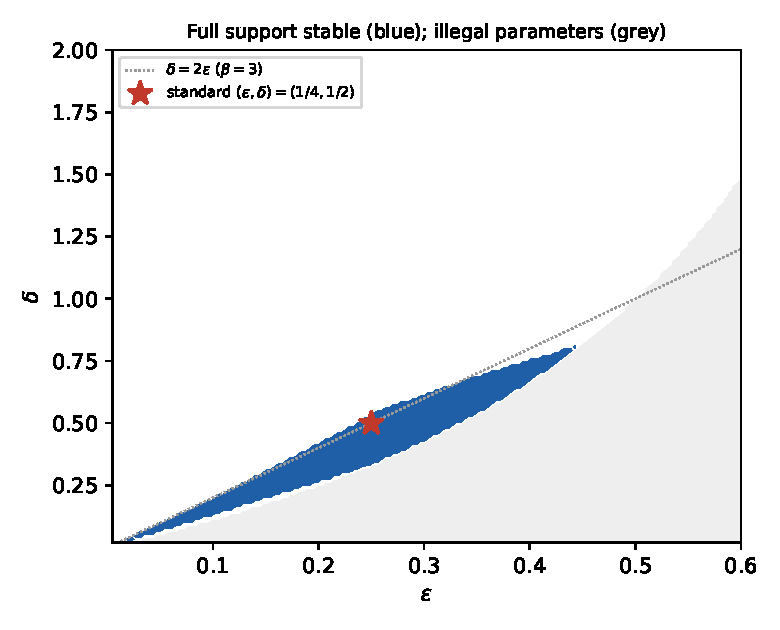
\includegraphics[width=.6\textwidth]{region.pdf}
\caption{Legal parameters at which the full support of $G_{\NSMALL}$ is a stable fixed point (blue), from a $160\times160$ floating-point grid; grey marks illegal parameters. The star is the standard point; the dotted line is $\delta=2\varepsilon$, that is $\beta=3$.}
\label{fig:region}
\end{figure}

\section{Verification}\label{sec:verify}

\texttt{check\_ctln.py} uses only the Python standard library. It builds $W$ from the arc list and checks legality and the nonclique property. It solves for $x^*$ over $\mathbb Q$ and checks the fixed-point identity exactly. It computes the characteristic polynomial of $K$ by a multimodular Hessenberg reduction with Chinese remaindering under a Hadamard bound, by Berkowitz's algorithm, and by rational Hessenberg reduction, and requires all three to agree. It then applies the Routh array and the Li\'enard-Chipart criterion, checks $K\equiv I\pmod3$, and for $n\le12$ also checks every principal and Cramer determinant directly. \texttt{check\_flint.py} is an independent implementation on FLINT through \texttt{python-flint}. It computes all $n$ Hurwitz determinants exactly. Both accept $G_{\NSMALL}$, $W_4$, and our 27- and 100-vertex examples. \texttt{check\_induced.py} performs the induced-subgraph check of part~(3) in exact arithmetic. The exhaustive search of Section~\ref{sec:exhaust} is replayed by \texttt{scan.sh}.

\section{What remains open}

\begin{itemize}
\item The exact minimum at the standard parameters, between $8$ and \NSMALL. Closing it needs either a search over the roughly $1.8\times10^{12}$ digraphs on eight vertices or a structural argument. \SPARSENOTE
\item Whether the conjecture fails at every legal parameter pair. In the large-$t$ limit, the families of \cite{CLTNrepo} reach $\beta$ close to $5$. Our own continuation stalled near $\beta\approx3.8$ at $t=3$.
\item The weaker conjecture of \cite{CGM2024}, that supports of stable fixed points are minimal in $\mathrm{FP}(W)$.
\end{itemize}

\paragraph{Research assistance.}
Valyu DeepResearch carried out literature and priority searches and adversarial reviews. These reviews are internal checks and do not constitute external peer review.

\bibliographystyle{plain}
\bibliography{references}
\end{document}
